\subsection{Scheduling energeticamente consapevole nelle piattaforme FaaS}
\label{subsec:energy_aware_scheduling}

Nel paradigma Function-as-a-Service (FaaS), lo scheduling non costituisce
soltanto un meccanismo di allocazione delle risorse, ma rappresenta uno
strumento strategico per il controllo del consumo energetico
dell'infrastruttura. A differenza delle politiche di pianificazione
tradizionali, orientate prevalentemente all'ottimizzazione delle
prestazioni o al bilanciamento del carico, lo scheduling energeticamente
consapevole integra il consumo energetico tra i criteri che guidano le
decisioni di \emph{placement} e la selezione delle risorse di esecuzione.

Nel contesto serverless, tale problematica presenta caratteristiche
peculiari legate al modello di esecuzione. La breve durata delle
funzioni, la loro natura stateless e l'isolamento in ambienti
containerizzati determinano un'elevata frequenza delle decisioni di
scheduling e una forte sensibilità alle condizioni operative del
momento. In particolare, l'inizializzazione di nuovi ambienti di
esecuzione (\emph{cold start}) può generare picchi di consumo energetico
istantaneo che influenzano in modo non trascurabile l'efficienza
complessiva del sistema; per questa ragione, la gestione del riutilizzo
degli ambienti già attivi (\emph{warm scheduling}) rappresenta una
dimensione rilevante tanto per la latenza percepita quanto per il
profilo energetico medio delle invocazioni.

Un ulteriore elemento di complessità è dato dalla natura distribuita
delle piattaforme FaaS, specialmente in architetture cloud-edge. In
questi scenari, i nodi disponibili per l'esecuzione possono differire
significativamente per capacità computazionale, profilo di consumo,
disponibilità energetica e connettività di rete. Le decisioni di
\emph{placement} devono quindi tenere conto non soltanto delle
prestazioni attese sul singolo nodo, ma anche delle condizioni
energetiche correnti dell'infrastruttura e, in alcuni casi, del costo
associato alla movimentazione dei dati tra siti eterogenei. Questa
molteplicità di fattori rende la progettazione di scheduler
energeticamente consapevoli per piattaforme FaaS un problema
intrinsecamente multi-dimensionale, nel quale le scelte progettuali
riflettono assunzioni diverse sull'architettura, sugli obiettivi di
ottimizzazione e sulle grandezze osservabili a runtime.

L'analisi della letteratura mostra come i contributi proposti in questo
ambito affrontino il problema operando su una leva decisionale comune
--- la scelta del nodo su cui eseguire la funzione --- ma declinandola
in funzione di scenari operativi distinti e con formulazioni
progressivamente più articolate. Nei paragrafi seguenti vengono
analizzati tre approcci rappresentativi, ciascuno dei quali evidenzia
una dimensione specifica della consapevolezza energetica nello scheduling
FaaS.

% ── Faashouse ──────────────────────────────────────────────────────────

In ambienti Edge Computing distribuiti, i nodi possono essere alimentati
da fonti rinnovabili intermittenti --- pannelli solari, micro-turbine
eoliche o batterie con autonomia limitata --- e presentare livelli di
carica variabili nel tempo. In tali contesti, l'obiettivo primario dello
scheduler non è la minimizzazione del consumo medio, bensì il
mantenimento dell'operatività dell'intero sistema, evitando che nodi
con disponibilità energetica residua insufficiente diventino
temporaneamente irraggiungibili o, nel caso peggiore, si spengano
durante l'esecuzione di una funzione.

Il sistema Faashouse~\cite{faashouse}, progettato per ambienti
serverless all'estremo edge, affronta questo problema adottando lo stato
di carica dei nodi (\emph{State of Charge}, SoC) come parametro
decisionale principale per le scelte di \emph{placement}. Come
illustrato in Figura~\ref{fig:faashouse_architecture}, l'architettura
si articola su più livelli --- dispositivi edge a bassa potenza,
piattaforma di containerizzazione e orchestrazione, e livello serverless
per la gestione delle funzioni --- con un \emph{Resource Scheduler}
integrato nel controller che implementa un ciclo di controllo
riconducibile al modello MAPE (\emph{Monitoring, Analyzing, Planning,
Execution}).

\begin{figure}[ht]
    \centering
    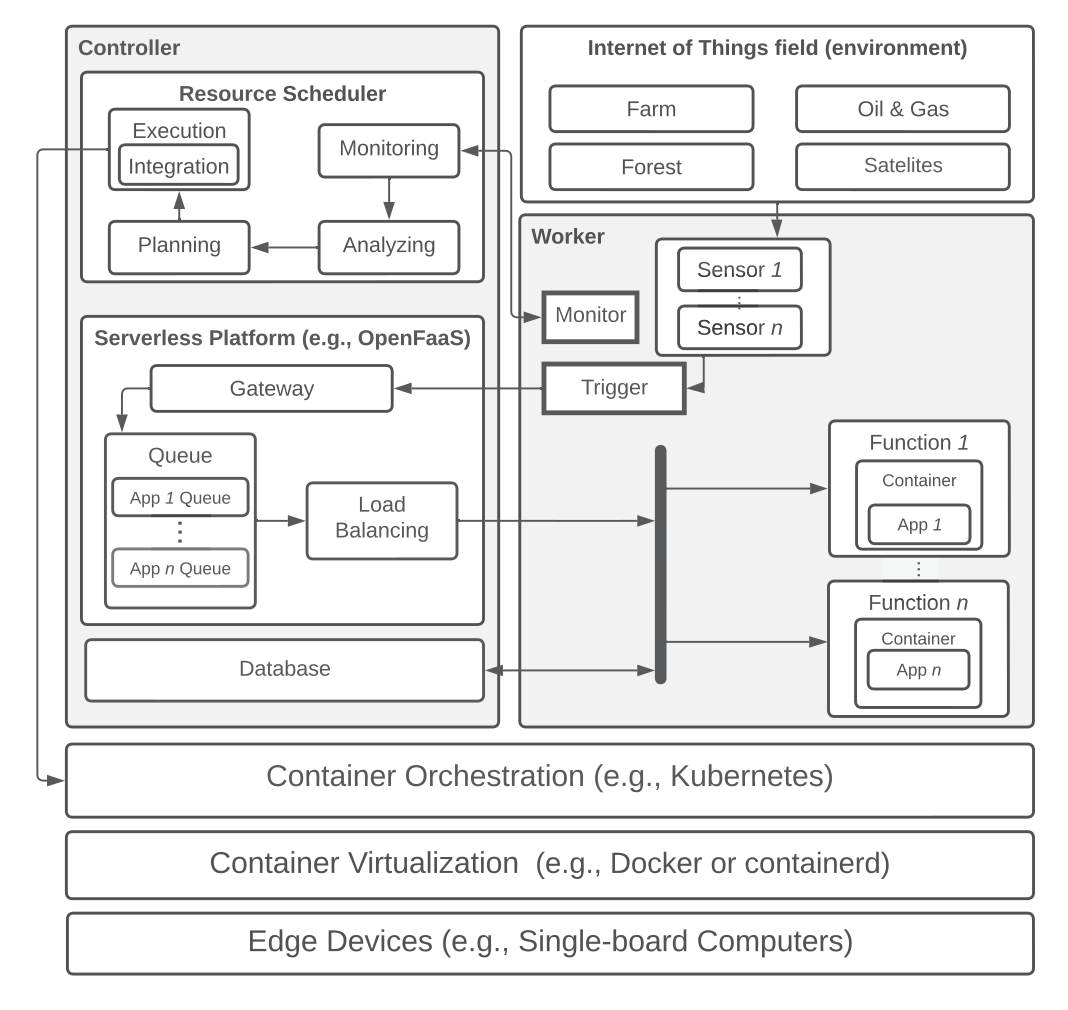
\includegraphics[width=0.9\textwidth]{figures/FaasHouse.png}
    \caption{Architettura del sistema Faashouse. Il controller integra un
    \emph{Resource Scheduler} che, seguendo un ciclo di monitoraggio,
    analisi e pianificazione, decide il \emph{placement} delle funzioni
    sui nodi worker in base allo stato energetico corrente.}
    \label{fig:faashouse_architecture}
\end{figure}

Lo stato energetico di ciascun nodo è una grandezza variabile nel tempo,
determinata congiuntamente dall'energia dissipata durante l'esecuzione
delle funzioni e dall'eventuale energia generata localmente dalle fonti
rinnovabili disponibili. Le decisioni di assegnazione incidono
direttamente sull'evoluzione di tale stato: concentrare le invocazioni
su nodi con SoC ridotto può comprometterne la disponibilità futura,
mentre una redistribuzione bilanciata consente di preservare
l'operatività complessiva dell'infrastruttura. Quando il livello di
carica di un nodo si avvicina a una soglia critica predefinita, le nuove
richieste vengono reindirizzate verso nodi con maggiore disponibilità
energetica mediante meccanismi di \emph{offloading}, realizzando un
bilanciamento energetico dinamico che si adatta alle condizioni
operative correnti.

Questo approccio risulta particolarmente efficace in scenari in cui la
principale fonte di variabilità è la disponibilità energetica
dell'infrastruttura piuttosto che il costo computazionale delle singole
funzioni. Faashouse opera infatti a granularità di nodo e non di
funzione: le invocazioni sono trattate come unità indivisibili, senza
distinzione tra funzioni con profili energetici differenti. Il consumo
energetico per invocazione non è un parametro su cui lo scheduler possa
agire; la sola leva disponibile è la redistribuzione del carico tra
nodi con diversa disponibilità di energia.

% ── E²FIS ──────────────────────────────────────────────────────────────

Se Faashouse affronta il problema della disponibilità energetica
distribuendo le invocazioni tra nodi con capacità residua sufficiente,
un approccio concettualmente diverso consiste nel ridurre il consumo
complessivo dell'infrastruttura attraverso il \emph{workload
consolidation}. In questo modello, lo scheduler non mira a distribuire
uniformemente il carico tra i nodi disponibili, bensì a concentrarlo su
un sottoinsieme selezionato, consentendo ai nodi rimanenti di essere
portati in stato inattivo e, di conseguenza, di non contribuire al
consumo energetico complessivo. L'intuizione alla base di questa
strategia è che il consumo di un nodo in stato di \emph{idle} --- pur
non eseguendo alcuna funzione --- rappresenta una quota non trascurabile
del budget energetico totale, e la sua eliminazione può produrre
risparmi significativi.

Un esempio rappresentativo di questo paradigma è E$^{2}$FIS
(\emph{Energy-Efficient Function Invocation Scheduling})~\cite{e2fis_smartcomp},
proposto per piattaforme FaaS nell'edge--cloud continuum. Il sistema
assume un insieme di nodi eterogenei, ciascuno caratterizzato da
capacità computazionale, memoria disponibile, throughput effettivo e
profilo di consumo energetico. Le funzioni sono descritte tramite
requisiti di memoria, carico computazionale e \emph{deadline} di
completamento; la stima del tempo di esecuzione tiene conto delle
differenze architetturali tra nodi, consentendo allo scheduler di
verificare la compatibilità di ciascuna assegnazione con i vincoli
temporali imposti.

\begin{figure}[ht]
    \centering
    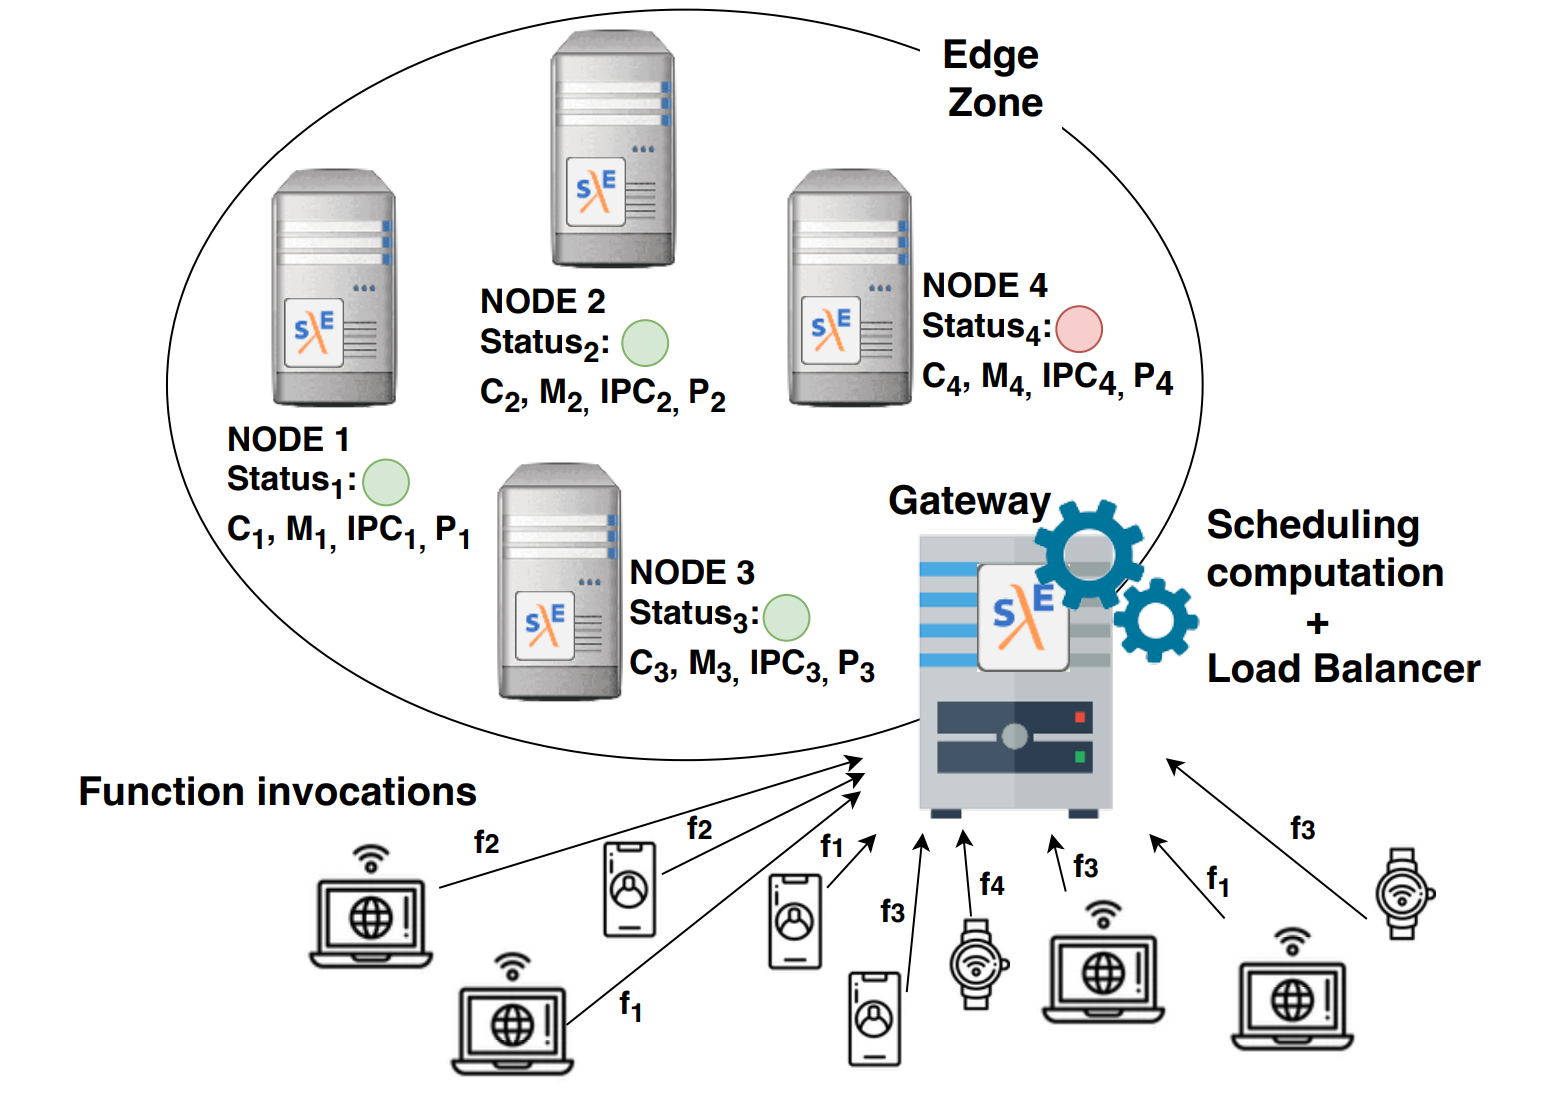
\includegraphics[width=0.85\textwidth]{figures/EnergyEfficientFunctionArchitecture.png}
    \caption{Architettura di E$^{2}$FIS. I nodi edge sono caratterizzati
    da differenti capacità computazionali e profili di consumo. Il modulo
    di \emph{Scheduling computation} determina periodicamente
    l'allocazione delle funzioni e il sottoinsieme di nodi da mantenere
    attivi.}
    \label{fig:e2fis_architecture}
\end{figure}

Come illustrato in Figura~\ref{fig:e2fis_architecture}, l'approccio
adotta una pianificazione periodica basata su epoche temporali discrete.
Prima dell'inizio di ciascuna epoca, il problema di allocazione viene
formulato come un'istanza di Programmazione Lineare Intera Mista (MILP)
e risolto offline. La funzione obiettivo minimizza il consumo energetico
associato ai nodi attivi nell'intervallo considerato, selezionando il
sottoinsieme minimo necessario a soddisfare tutte le richieste entro le
rispettive deadline. Ne deriva una logica di consolidamento: quando il
carico complessivo lo consente, le invocazioni vengono concentrate sui
nodi con il miglior rapporto tra capacità computazionale e consumo
energetico, mentre i restanti possono essere portati in stato inattivo.

Per garantire robustezza operativa in presenza di istanze
computazionalmente onerose o di vincoli particolarmente stringenti, il
sistema prevede un limite temporale per la risoluzione del problema di
ottimizzazione: qualora la soluzione ottima non sia ottenibile entro la
soglia stabilita, viene adottata la migliore soluzione ammissibile
disponibile. In condizioni limite, il framework può inoltre ricorrere a
una politica di fallback ispirata a EDF (\emph{Earliest Deadline
First}), privilegiando il rispetto delle deadline rispetto
all'ottimizzazione energetica. Tale meccanismo evidenzia come, nella
progettazione di scheduler energy-aware, il rispetto dei vincoli
temporali costituisca un obiettivo che, in situazioni di sovraccarico,
assume priorità rispetto all'efficienza energetica, introducendo una
gerarchia esplicita tra gli obiettivi del sistema.

Rispetto a Faashouse, E$^{2}$FIS opera su una leva diversa: anziché
redistribuire il carico in base allo stato energetico corrente dei nodi,
interviene sulla topologia stessa dell'infrastruttura attiva, riducendo
il numero di elementi che contribuiscono al consumo complessivo. Anche
in questo caso, tuttavia, il perimetro decisionale rimane circoscritto
al livello infrastrutturale: lo scheduler seleziona i nodi e assegna le
invocazioni, senza intervenire sulla logica applicativa delle funzioni
eseguite.

% ── GreenFaaS ──────────────────────────────────────────────────────────

I due approcci esaminati finora operano nell'ipotesi che le funzioni
vengano eseguite sullo stesso sito in cui risiedono i dati di input,
o che il costo della loro movimentazione sia trascurabile. In ambienti
FaaS federati o multi-sito, tuttavia, questa assunzione non è sempre
valida. Quando risorse eterogenee e geograficamente distribuite --- tra
cui cluster HPC, workstation e infrastrutture cloud --- partecipano alla
stessa piattaforma di esecuzione, le funzioni possono operare su dataset
residenti in domini amministrativi distinti. In tali scenari, la
decisione di \emph{placement} non dipende soltanto dall'efficienza del
nodo di calcolo, ma anche dal costo energetico necessario a rendere
disponibili i dati di input nel sito selezionato. Ne consegue che
l'allocazione ottimale deve considerare congiuntamente il costo di
\emph{computation} e di \emph{communication}, evitando scelte che
riducono il consumo di esecuzione introducendo al contempo overhead
energetici significativi dovuti alla movimentazione dei dati.

In questo contesto si colloca GreenFaaS~\cite{greenfaas}, un framework
progettato per orchestrare invocazioni FaaS in ambienti distribuiti,
integrando nella decisione di scheduling una stima esplicita del costo
energetico dei trasferimenti. Come mostrato in
Figura~\ref{fig:greenfaas_arch}, l'architettura si articola in tre
componenti principali: un modulo di \emph{Resource Monitoring}, un
\emph{Transfers Manager} e uno \emph{Scheduler}.

\begin{figure}[ht]
    \centering
    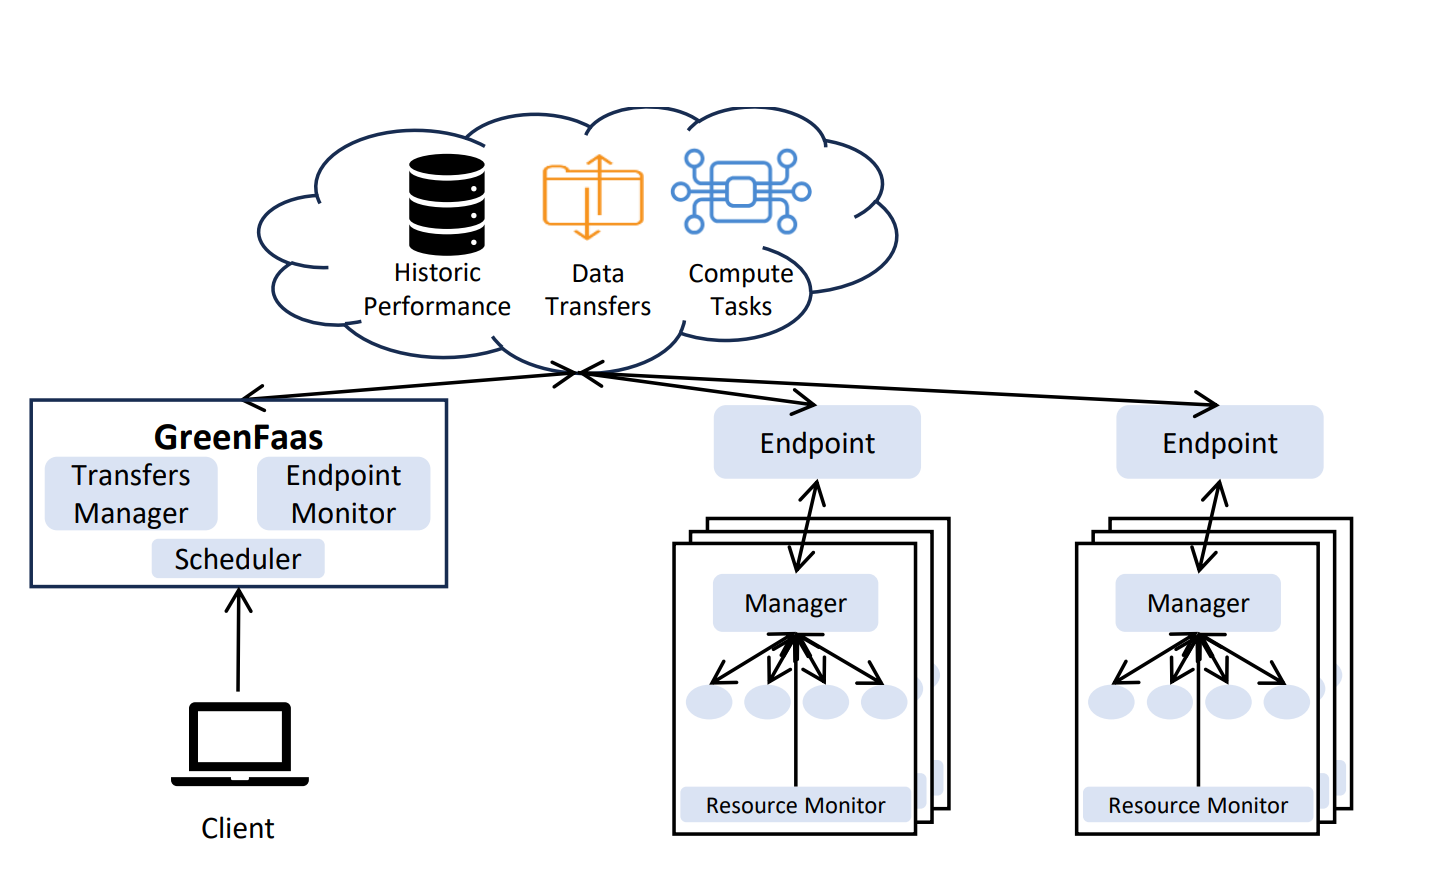
\includegraphics[width=0.9\textwidth]{figures/GreenFaas.png}
    \caption{Architettura di alto livello di GreenFaaS: monitoraggio degli
    endpoint, stima del costo energetico dei trasferimenti e scheduling
    energy-aware per l'allocazione dei task in ambienti federati
    eterogenei.}
    \label{fig:greenfaas_arch}
\end{figure}

Il modulo di monitoraggio raccoglie a runtime metriche energetiche e
prestazionali dei nodi, sfruttando interfacce hardware --- tra cui RAPL
per CPU e NVML per GPU --- per derivare stime di potenza e
caratterizzare il comportamento energetico delle risorse disponibili.
Tali misure consentono di stimare il costo di esecuzione su piattaforme
eterogenee, riducendo la dipendenza da proxy indiretti quali il solo
tempo di esecuzione. Il \emph{Transfers Manager}, a sua volta, modella
il contributo energetico associato alla movimentazione dei dati tra
siti: quando l'input risiede in un dominio diverso da quello candidato
all'esecuzione, il trasferimento introduce un costo legato alla
trasmissione in rete e alle operazioni di I/O agli estremi della
comunicazione. GreenFaaS stima tale costo in funzione della dimensione
dei dati e delle caratteristiche del collegamento, consentendo di
quantificare l'impatto energetico della scelta del sito anche nei casi
in cui il nodo remoto risulti computazionalmente più efficiente.

Sulla base di queste informazioni, lo \emph{Scheduler} effettua una
selezione multi-criterio che integra il consumo energetico previsto per
l'esecuzione sul nodo candidato e il costo energetico dei trasferimenti
eventualmente necessari, affiancando a tali grandezze una stima del
tempo di completamento. Il peso relativo delle componenti è
configurabile, consentendo di modulare il compromesso tra efficienza
energetica e prestazioni in funzione degli obiettivi applicativi. Per
mantenere la reattività in presenza di carichi dinamici e
infrastrutture di grandi dimensioni, il framework adotta strategie
euristiche che evitano un'ottimizzazione globale onerosa.

GreenFaaS amplia dunque la nozione di consapevolezza energetica nello
scheduling FaaS oltre la sola scelta del nodo computazionale,
estendendola al costo di comunicazione tra siti. Questo contributo è
particolarmente rilevante in architetture federali con forte dispersione
geografica, dove i trasferimenti dati possono incidere significativamente
sul bilancio energetico complessivo.

% ── Osservazioni conclusive ────────────────────────────────────────────

Nel complesso, i tre approcci analizzati condividono un elemento
strutturale comune: la decisione di scheduling opera esclusivamente
sulla scelta del nodo di esecuzione, trattando la funzione invocata
come un'entità atomica con un profilo energetico dato. Faashouse
redistribuisce il carico in base alla disponibilità energetica residua
dei nodi; E$^{2}$FIS concentra le invocazioni su un sottoinsieme di
nodi selezionato per minimizzare il consumo complessivo;
GreenFaaS estende la valutazione al costo di comunicazione in ambienti
multi-sito. In nessuno di questi approcci il consumo per singola
invocazione è un parametro su cui lo scheduler possa intervenire: la
funzione viene eseguita nella sua forma originale, indipendentemente
dalle condizioni energetiche del sistema al momento dell'invocazione.

Questa osservazione delimita l'ambito di applicabilità degli approcci
infrastrutturali e motiva l'interesse verso soluzioni che operino a un
livello diverso dello stack di esecuzione, agendo sulla logica
applicativa della funzione piuttosto che sulla selezione del nodo.
Tale direzione è esplorata nelle sezioni successive attraverso il
paradigma dell'Approximate Computing.